\documentclass[12pt]{article}
%	options include 12pt or 11pt or 10pt
%	classes include article, report, book, letter, thesis
\usepackage{amsmath} 
\usepackage{amstext} 
\usepackage{graphicx}

   

\title{This is the title}
\author{Author One \\ Author Two}
\date{29 February 2004}

\begin{document}
\maketitle

\section{EBM}

Energy-Based Models (EBM)
Energy-based models associate a scalar energy to each configuration of the variables of interest. Learning corresponds to modifying that energy function so that its shape has desirable properties. For example, we would like plausible or desirable configurations to have low energy. Energy-based probabilistic models define a probability distribution through an energy function, as follows:
\begin{equation}
(1)p(x) = \frac {e^{-E(x)}} {Z}.
\end{equation}


The normalizing factor Z is called the partition function by analogy with physical systems.
\begin{equation}
Z = \sum_x e^{-E(x)}
\end{equation}


An energy-based model can be learnt by performing (stochastic) gradient descent on the empirical negative log-likelihood of the training data. As for the logistic regression we will first define the log-likelihood and then the loss function as being the negative log-likelihood.

\begin{equation}
\mathcal{L}(\theta, \mathcal{D}) = \frac{1}{N} \sum_{x^{(i)} \in
\mathcal{D}} \log\ p(x^{(i)})\\
\ell (\theta, \mathcal{D}) = - \mathcal{L} (\theta, \mathcal{D})
\end{equation}


using the stochastic gradient $-\frac{\partial  \log p(x^{(i)})}{\partial 
\theta}$ , where $\theta$ are the parameters of the model.




EBMs with Hidden Units

In many cases of interest, we do not observe the example x fully, or we want to introduce some non-observed variables to increase the expressive power of the model. So we consider an observed part (still denoted x here) and a hidden part h. We can then write:
\begin{equation}
P(x) = \sum_h P(x,h) = \sum_h \frac{e^{-E(x,h)}}{Z}.
\end{equation}

In such cases, to map this formulation to one similar to Eq. (1), we introduce the notation (inspired from physics) of free energy, defined as follows:
\begin{equation}
\mathcal{F}(x) = - \log \sum_h e^{-E(x,h)}
\end{equation}
which allows us to write,

\begin{equation}
P(x) = \frac{e^{-\mathcal{F}(x)}}{Z} \text{ with } Z=\sum_x e^{-\mathcal{F}(x)}.
\end{equation}
The data negative log-likelihood gradient then has a particularly interesting form.

\begin{equation}
- \frac{\partial  \log p(x)}{\partial \theta}
= \frac{\partial \mathcal{F}(x)}{\partial \theta} -
       \sum_{\tilde{x}} p(\tilde{x}) \
           \frac{\partial \mathcal{F}(\tilde{x})}{\partial \theta}.
\end{equation}

Notice that the above gradient contains two terms, which are referred to as the positive and negative phase. The terms positive and negative do not refer to the sign of each term in the equation, but rather reflect their effect on the probability density defined by the model. The first term increases the probability of training data (by reducing the corresponding free energy), while the second term decreases the probability of samples generated by the model.

It is usually difficult to determine this gradient analytically, as it involves the computation of $E_P$ \[ \frac{\partial \mathcal{F}(x)} {\partial \theta} \] . This is nothing less than an expectation over all possible configurations of the input x (under the distribution P formed by the model) !

The first step in making this computation tractable is to estimate the expectation using a fixed number of model samples. Samples used to estimate the negative phase gradient are referred to as negative particles, which are denoted as $\mathcal{N}$. The gradient can then be written as:

\begin{equation}
(5)- \frac{\partial \log p(x)}{\partial \theta}
 \approx
  \frac{\partial \mathcal{F}(x)}{\partial \theta} -
   \frac{1}{|\mathcal{N}|}\sum_{\tilde{x} \in \mathcal{N}} \
   \frac{\partial \mathcal{F}(\tilde{x})}{\partial \theta}.
\end{equation}

where we would ideally like elements $\tilde{x}$ of $\mathcal{N}$ to be sampled according to P (i.e. we are doing Monte-Carlo). With the above formula, we almost have a pratical, stochastic algorithm for learning an EBM. The only missing ingredient is how to extract these negative particles $\mathcal{N}$. While the statistical literature abounds with sampling methods, Markov Chain Monte Carlo methods are especially well suited for models such as the Restricted Boltzmann Machines (RBM), a specific type of EBM.

\section{RBM}

Boltzmann Machines (BMs) are a particular form of log-linear Markov Random Field (MRF), i.e., for which the energy function is linear in its free parameters. To make them powerful enough to represent complicated distributions (i.e., go from the limited parametric setting to a non-parametric one), we consider that some of the variables are never observed (they are called hidden). By having more hidden variables (also called hidden units), we can increase the modeling capacity of the Boltzmann Machine (BM). Restricted Boltzmann Machines further restrict BMs to those without visible-visible and hidden-hidden connections. A graphical depiction of an RBM is shown below.


\begin{figure}
	\centering
	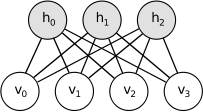
\includegraphics[width=0.74\textwidth]
		{pics/rbm.png}
	\caption{gambar RBM}
	\label{fig:lisensi}
\end{figure}


The energy function E(v,h) of an RBM is defined as:

\begin{equation}
E(v,h) = - b'v - c'h - h'Wv
\end{equation}

where W represents the weights connecting hidden and visible units and b, c are the offsets of the visible and hidden layers respectively.

This translates directly to the following free energy formula:

\begin{equation}
\mathcal{F}(v)= - b'v - \sum_i \log \sum_{h_i} e^{h_i (c_i + W_i v)}.
\end{equation}

Because of the specific structure of RBMs, visible and hidden units are conditionally independent given one-another. Using this property, we can write:

\begin{equation}
p(h|v) \&= \prod_i p(h_i|v) \\
p(v|h) \&= \prod_j p(v_j|h).
\end{equation}

RBMs with binary units

In the commonly studied case of using binary units (where $v_j$ and $h_i$ $\in
\{0,1\}$), we obtain from Eq. (6) and (2), a probabilistic version of the usual neuron activation function:

\begin{equation}
(7)P(h_i=1|v) = sigm(c_i + W_i v) \\
\end{equation}

\begin{equation}
(8)P(v_j=1|h) = sigm(b_j + W'_j h)
\end{equation}

The free energy of an RBM with binary units further simplifies to:

\begin{equation}
(9)\mathcal{F}(v)= - b'v - \sum_i \log(1 + e^{(c_i + W_i v)}).
\end{equation}
Update Equations with Binary Units

Combining Eqs. (5) with (9), we obtain the following log-likelihood gradients for an RBM with binary units:

\begin{equation}
(10)- \frac{\partial{ \log p(v)}}{\partial W_{ij}} \&=
    E_v[p(h_i|v) \cdot v_j]
    - v^{(i)}_j \cdot sigm(W_i \cdot v^{(i)} + c_i) \\
-\frac{\partial{ \log p(v)}}{\partial c_i} \&=
    E_v[p(h_i|v)] - sigm(W_i \cdot v^{(i)})  \\
-\frac{\partial{ \log p(v)}}{\partial b_j} \&=
    E_v[p(v_j|h)] - v^{(i)}_j
\end{equation}

For a more detailed derivation of these equations, we refer the reader to the following page, or to section 5 of Learning Deep Architectures for AI. We will however not use these formulas, but rather get the gradient using Theano T.grad from equation (4).

Sampling in an RBM
Samples of $p(x)$ can be obtained by running a Markov chain to convergence, using Gibbs sampling as the transition operator.

Gibbs sampling of the joint of N random variables $S=(S_1, ... , S_N)$ is done through a sequence of N sampling sub-steps of the form $S_i \sim p(S_i | S_{-i})$ where $S_{-i}$ contains the $N-1$ other random variables in $S$ excluding $S_i$.

For RBMs, S consists of the set of visible and hidden units. However, since they are conditionally independent, one can perform block Gibbs sampling. In this setting, visible units are sampled simultaneously given fixed values of the hidden units. Similarly, hidden units are sampled simultaneously given the visibles. A step in the Markov chain is thus taken as follows:

\begin{equation}
h^{(n+1)} \&\sim sigm(W'v^{(n)} + c) \\
v^{(n+1)} \&\sim sigm(W h^{(n+1)} + b),
\end{equation}

where $h^{(n)}$ refers to the set of all hidden units at the n-th step of the Markov chain. What it means is that, for example, $h^{(n+1)}_i$ is randomly chosen to be 1 (versus 0) with probability $sigm(W_i'v^{(n)} + c_i)$, and similarly, $v^{(n+1)}_j$ is randomly chosen to be 1 (versus 0) with probability $sigm(W_{.j} h^{(n+1)} + b_j)$.

This can be illustrated graphically:

$images/markov_chain.png$
As t $\rightarrow \infty$, samples $(v^{(t)}, h^{(t)})$ are guaranteed to be accurate samples of $p(v,h)$.

In theory, each parameter update in the learning process would require running one such chain to convergence. It is needless to say that doing so would be prohibitively expensive. As such, several algorithms have been devised for RBMs, in order to efficiently sample from $p(v,h)$ during the learning process.

Contrastive Divergence (CD-k)
Contrastive Divergence uses two tricks to speed up the sampling process:

since we eventually want $p(v) \approx p_{train}(v)$ (the true, underlying distribution of the data), we initialize the Markov chain with a training example (i.e., from a distribution that is expected to be close to p, so that the chain will be already close to having converged to its final distribution p).
CD does not wait for the chain to converge. Samples are obtained after only k-steps of Gibbs sampling. In pratice, k=1 has been shown to work surprisingly well.
Persistent CD
Persistent CD [Tieleman08] uses another approximation for sampling from p(v,h). It relies on a single Markov chain, which has a persistent state (i.e., not restarting a chain for each observed example). For each parameter update, we extract new samples by simply running the chain for k-steps. The state of the chain is then preserved for subsequent updates.

The general intuition is that if parameter updates are small enough compared to the mixing rate of the chain, the Markov chain should be able to “catch up” to changes in the model.

Implementation
We construct an RBM class. The parameters of the network can either be initialized by the constructor or can be passed as arguments. This option is useful when an RBM is used as the building block of a deep network, in which case the weight matrix and the hidden layer bias is shared with the corresponding sigmoidal layer of an MLP network.

% terjemahan :

Energy-Based Models (EBM)
EBM mengaitkan sebuah energi skalar pada setiap konfigurasi variable yang diingini. Proses learning bertujuan untuk memodifikasi fungsi energi sehingga bentuknya memiliki  sifat yang diinginkan. Sebagai contoh, misalnya diinginkan sebuah bentuk konfigurasi yang memiliki energi yang rendah, maka model probabilistik dari EBM didifinisikan sebagi distribusi probabilitas melalui fungsi energi sebagi berikut:

(1)p(x) = \frac {e^{-E(x)}} {Z}.
\end{document}
